 \documentclass[12pt,a4paper,titlepage]{article}
\usepackage[utf8]{inputenc}
\usepackage[finnish]{babel}
\usepackage{setspace}
\usepackage{subcaption}
\usepackage{fancyhdr}
\usepackage[top=1in, bottom=1in, left=1in, right=1in]{geometry}
\usepackage{float}
\usepackage{pdfpages}
\usepackage{enumitem}
\usepackage{tabularx}

\usepackage{hyperref}
\hypersetup{pdfborder={0 0 0}}
\onehalfspacing
\cfoot{}
\rhead{\thepage}
\lhead{\leftmark}

\title{Tsoha\\ Kurssikysely \vspace{0.5em}}
\author{Anni Järvenpää}
\date{\today}

\begin{document}
\maketitle

% Sisällysluettelo
\newpage
\tableofcontents
\thispagestyle{empty}
\newpage
\setcounter{page}{1}
\parskip=1em \advance\parskip by 0pt plus 2pt
\pagestyle{fancy}
\cfoot{\thepage}

%%%%%%%%%%%%%%% Oleellinen sisältö alkaa%%%%%%%%%%%%%%%
\section{Johdanto}
Työn tavoitteena on toteuttaa kurssikyselyjärjestelmä, jonka avulla opiskelijoilta voidaan kerätä palautetta kursseista. Järjestelmää voidaan käyttää koko tiedekunnassa ja kyselyt sisältävätkin sekä koko tiedekunnan laajuisia kysymyksiä että laitos- ja kurssikohtaisia kysymyksiä. Kysymysten vastaukset voivat olla avoimia tai ne voidaan valita numeroasteikolta tai muusta annetusta arvojoukosta.

Kurssin luennoitsija voi lisätä, poistaa ja muokata kurssikohtaisia kysymyksiä ja laitoksen ja tiedekunnan hallintohenkilöstö niiden kysymyksiä. Samoin uusille kursseille voidaan luoda uusia kyselyitä ja vanhoja voidaan poistaa. Kyselyn muokkaaminen tai poistaminen edellyttää kuitenkin, ettei kysely ole parhaillaan käynnissä.

Laitos ja tiedekunta voivat hakea yhteenvedon kurssin tai kurssien kysymysten tuloksista kuten vastaajamääristä tai tiettyyn kysymykseen saaduista vastauksista. Kurssin pitäjä saa järjestelmästä yksityiskohtaisen raportin kyselyn tuloksista aina halutessaan.


\section{Yleiskuva järjestelmästä}
Järjestelmää käyttävät opiskelijat, opettajat ja laitoksen sekä tiedekunnan hallintohenkilöt. Näistä kaikki voivat kirjautua järjestelmään ja tarkastella kyselyitä. Näkyvät kyselyt ja niille tehtävissä olevat operaatiot riippuvat kuitenkin käyttäjäryhmästä. Käyttö\-tapaus\-kaavio on nähtävillä kuvassa \ref{fig:kayttotapauskaavio} ja käyttötapaukset on eritelty alla.

\begin{figure}
   \centering
   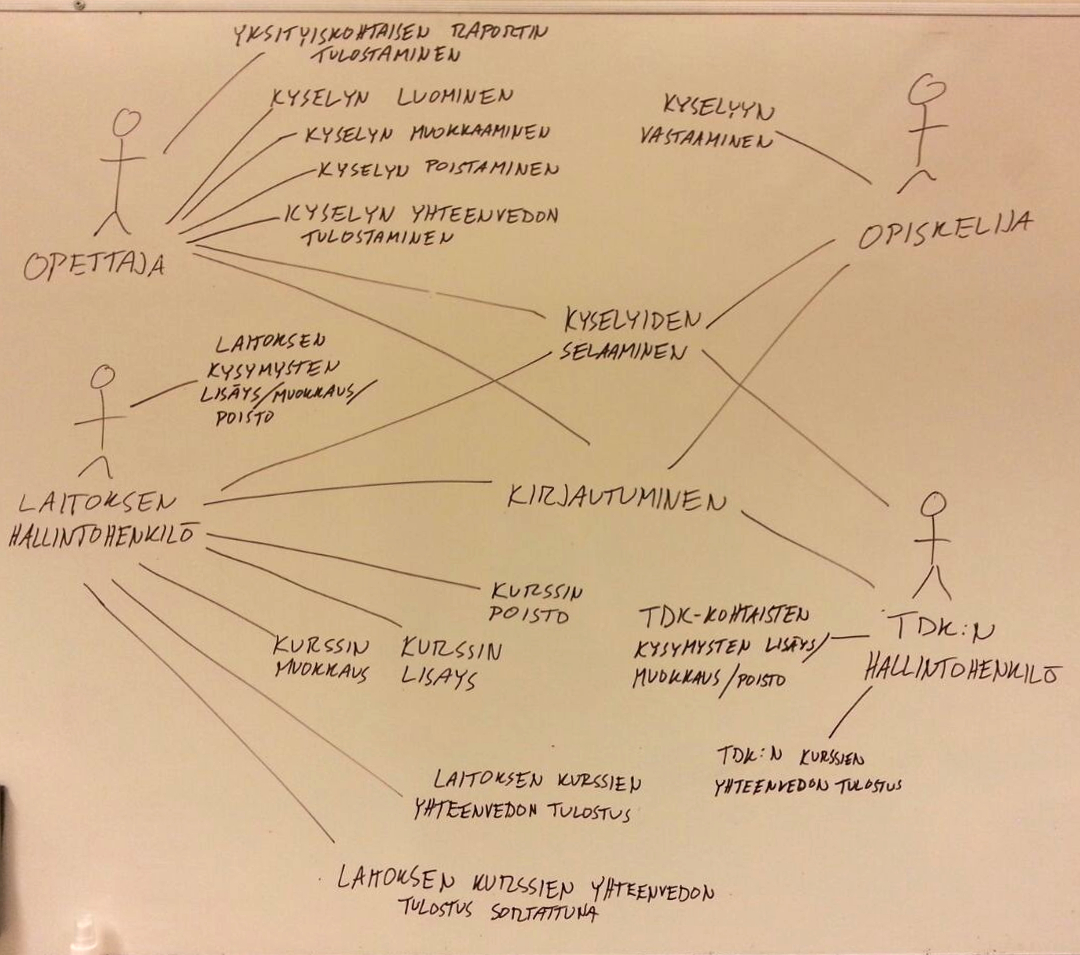
\includegraphics[width=\textwidth]{kuvat/kayttotapauskaavio.jpg}
   \caption{Järjestelmän käyttötapauskaavio}\label{fig:kayttotapauskaavio}
\end{figure}

\begin{description}[style=nextline]
    \item[Kirjautuminen] Kaikki käyttäjäryhmät voivat kirjautua palveluun ja palvelun käyttäminen alkaa aina kirjautumisella.
    \item[Kyselyiden selaaminen] Kirjautumisen jälkeen käyttäjä viedään selaamaan kyselyitä. Näytettävien kyselyjen määrä ja kyselyistä näytettävät tiedot riippuvat käyttäjäryhmästä.
    \item[Yksityiskohtaisen kyselyraportin näyttäminen] Opettaja voi pyytää kyselystä yksityiskohtaisen raportin. Tällöin hänelle näytetään kurssin perustiedot, kyselyn status ja vastausten lukumäärä. Tästä näkymästä pääsee myös lisäämään, muokkaamaan ja poistamaan kyselyitä.
    \item[Kyselyn luominen] Opettaja pystyy luomaan opettamalleen kurssille kyselyn. Tällöin avataan tyhjä kysely muokkaustilassa.
    \item[Kyselyn muokkaaminen] Opettaja voi muokata oman kyselynsä kysymyksiä. Tällöin hänelle näytetään lista nykyisistä kysymyksistä ja annetaan mahdollisuus poistaa niitä tai siirtyä luomaan uusia tai muokkaamaan vanhoja. Kyselyn muokkaaminen ei onnistu enää kun kysely on avattu opiskelijoille.
    \item[Kyselyn tilan muuttaminen] Kurssin opettaja voi muuttaa kyselyn tilan luonnoksesta käynnissä olevaksi, jolloin opiskelijat voivat vastata kyselyyn, tai käynnissä olevasta päättyneeksi, jolloin kyselyyn ei voi enää vastata mutta kyselyn tiedot ovat hallintohenkilöiden nähtävissä.
    \item[Kysymyksen lisääminen (opettaja)] Kysymystä lisättäessä opettaja voi antaa kysymyksen ja valita sen tyypin sekä monivalintakysymystä luotaessa vastausvaihtoehdot.
    \item[Kysymyksen muokkaaminen (opettaja)] Kysymyksen muokkaaminen toimii vastaavasti kuin kysymyksen lisääminen, mutta oletusarvoina käytetään kysymyksen nykytilaa.
    \item[Kysymyksen lisääminen (hallinto)] Kysymystä lisättäessä hallintohenkilöiltä kysytään ainoastaan kysymystä, sillä vastaukset ovat aina numeerisia standardiasteikolla.
    \item[Kysymyksen poistaminen] Opettajat sekä hallintohenkilöt voivat poistaa oman organisaatiotasonsa/kyselynsä kysymyksiä. Kysymyksen poistaminen täytyy vahvistaa klikkaamalla ennen poiston astumista voimaan.
    \item[Kurssin lisääminen] Laitoksen hallintohenkilöt voivat lisätä kursseja. Tällöin kurssista annetaan sen nimi, opettaja tai opettajat, kurssin alkamis- ja päättymispäivät ja mahdollisesti linkki kurssin kotisivulle.
    \item[Kurssin muokkaaminen] Laitoksen hallintohenkilöt voivat muokata kurssien tietoja niistä kursseista, joilla ei ole kyselyitä, jotka olisivat olleet vastattavissa.
    \item[Kurssin poistaminen] Laitoksen hallintohenkilöt voivat poistaa kursseja, joilla ei ole vielä kyselyä, joka olisi ollut vastattavissa.
    \item[Laitoskohtaisten kysymysten tulosten tarkastelu] Laitoskohtaisten kysymysten vastausten keskiarvot ja vastausprosentit näytetään kursseittain. Tämä näkymä on saatavilla laitoksen ja tiedekunnan hallintohenkilöille.
    \item[Tiedekuntakohtaisten kysymysten tulosten tarkastelu] Laitoskohtaisten kysymysten vastausten keskiarvot ja vastausprosentit näytetään kursseittain. Tämä näkymä on saatavilla tiedekunnan hallintohenkilöille.
    \item[Laitoskohtaisten kysymysten lisääminen] Laitoksen hallintohenkilöt voivat lisätä laitoskohtaisia kysymyksiä syöttämällä haluttu kysymys tekstikenttään.
    \item[Laitoskohtaisten kysymysten muokkaaminen] Laitoksen hallintohenkilöt voivat muokata laitoskohtaisia kysymyksiä.
    \item[Laitoskohtaisten kysymysten poistaminen] Laitoksen hallintohenkilöt voivat poistaa laitoskohtaisia kysymyksiä. Poistaminen vahvistetaan dialogilla.
    \item[Tiedekuntakohtaisten kysymysten lisääminen] Laitoksen hallintohenkilöt voivat lisätä laitoskohtaisia kysymyksiä syöttämällä haluttu kysymys tekstikenttään.
    \item[Tiedekuntakohtaisten kysymysten muokkaaminen] Laitoksen hallintohenkilöt voivat muokata laitoskohtaisia kysymyksiä.
    \item[Tiedekuntakohtaisten kysymysten poistaminen] Laitoksen hallintohenkilöt voivat poistaa laitoskohtaisia kysymyksiä. Poistaminen vahvistetaan dialogilla.    
\end{description}

%Jokaisen käyttäjäryhmän käyttäjät voivat kirjautua palveluun ja selata kyselyitä. Käyttäjälle näytettävä valikoima kuitenkin vaihtelee: opiskelija näkee ainoastaan avoimet kyselyt niiltä kursseilta, joilla on osallistujana, opettaja ainoastaan omien kurssiensa kyselyt ja laitoksen hallintohenkilöt ainoastaan oman laitoksen kurssit. Tiedekunnan hallintohenkilöt puolestaan näkevät kaikkien kurssien kyselyt. Kyselyihin pystyy vastaamaan ainoastaan opiskelija.
%
%Tiedekuntakohtaisten kysymysten luomisesta sekä tarvittaessa muokkaamisesta ja poistamisesta vastaa tiedekunnan hallintohenkilö. Tätä varten kysymykset on toki voitava myös listata, vaikka sitä ei ole piirretty näkyviin käyttötapauskaavioon. Lisäksi tiedekunnan hallintohenkilö voi tulostaa nähtävilleen yhteenvedon kyselyiden tuloksista.
%
%Laitoksen hallintohenkilöt vastaavat laitoskohtaisten kysymysten luomisesta, muokkaamisesta ja poistamisesta. Heidän tehtävänään on pitää esimerkiksi kurssin vastuuopettajatiedot ajantasaisina. Lisäksi he luovat uudet kurssit ja hoitavat muuttuneiden kurssitietojen muokkaamisen tai valikoimasta poistuneiden kurssien poistamisen. Vastaavasti kuin tiedekuntakohtaisissa kysymyksissä, laitoksen hallintohenkilöt voivat tarkastella laitoskohtaisiin kysymyksiin saatujen vastausten yhteenvetoja.
%
%Kurssin opettaja voi lisätä omille kursseilleen kyselyitä. Niitä voi myös muokata tai poistaa, ei kuitenkaan silloin, kun ne ovat avoimina eli opiskelijat voivat vastana niihin. Myös opettaja voi pyytää yhteenvetoraportin jonkin kyselyn tuloksista. Koska esimerkiksi tekstimuotoisten kysymysten tapauksessa on yksittäisten vastausten tarkasteleminen tarpeen, voidaan myös yksittäisen kurssin kyselyn kaikki vastaukset näyttää yksityiskohtaisessa raportissa.
%
%Yhteenvetoraporttia tulostettaessa laitoksen ja tiedekunnan hallintohenkilöt näkevät aina omalle organisaatiotasolleen spesifien kysymysten vastausten keskiarvot ja -hajonnat sekä vastaajamäärät. Näkymä voidaan haluttaessa järjestää tietyn kysymyksen vastausten perusteella. Tästä syystä tiedekunta- tai laitoskohtaisten kysymysten vastaukset voivat olla ainoastaan numeerisia.
%
%Vastaavasti opettaja voi tulostaa yhteenvetoraportin tietyn kyselyn vastauksista, jolloin hän saa nähtäväkseen kustakin kyselyn kysymyksestä vastauksien keskiarvon ja keskihajonnan. Opettaja voi halutessaan tarkastella myös yksityiskohtaisia raportteja kursseistaan, jolloin hän saa nähtäväkseen kyselyn kunkin kysymyksen vastausjakauman (monivalintakysymykset) tai kaikki annetut vastaukset (aviomet kysymykset).

\section{Järjestelmän tietosisältö}
\begin{figure}
   \centering
   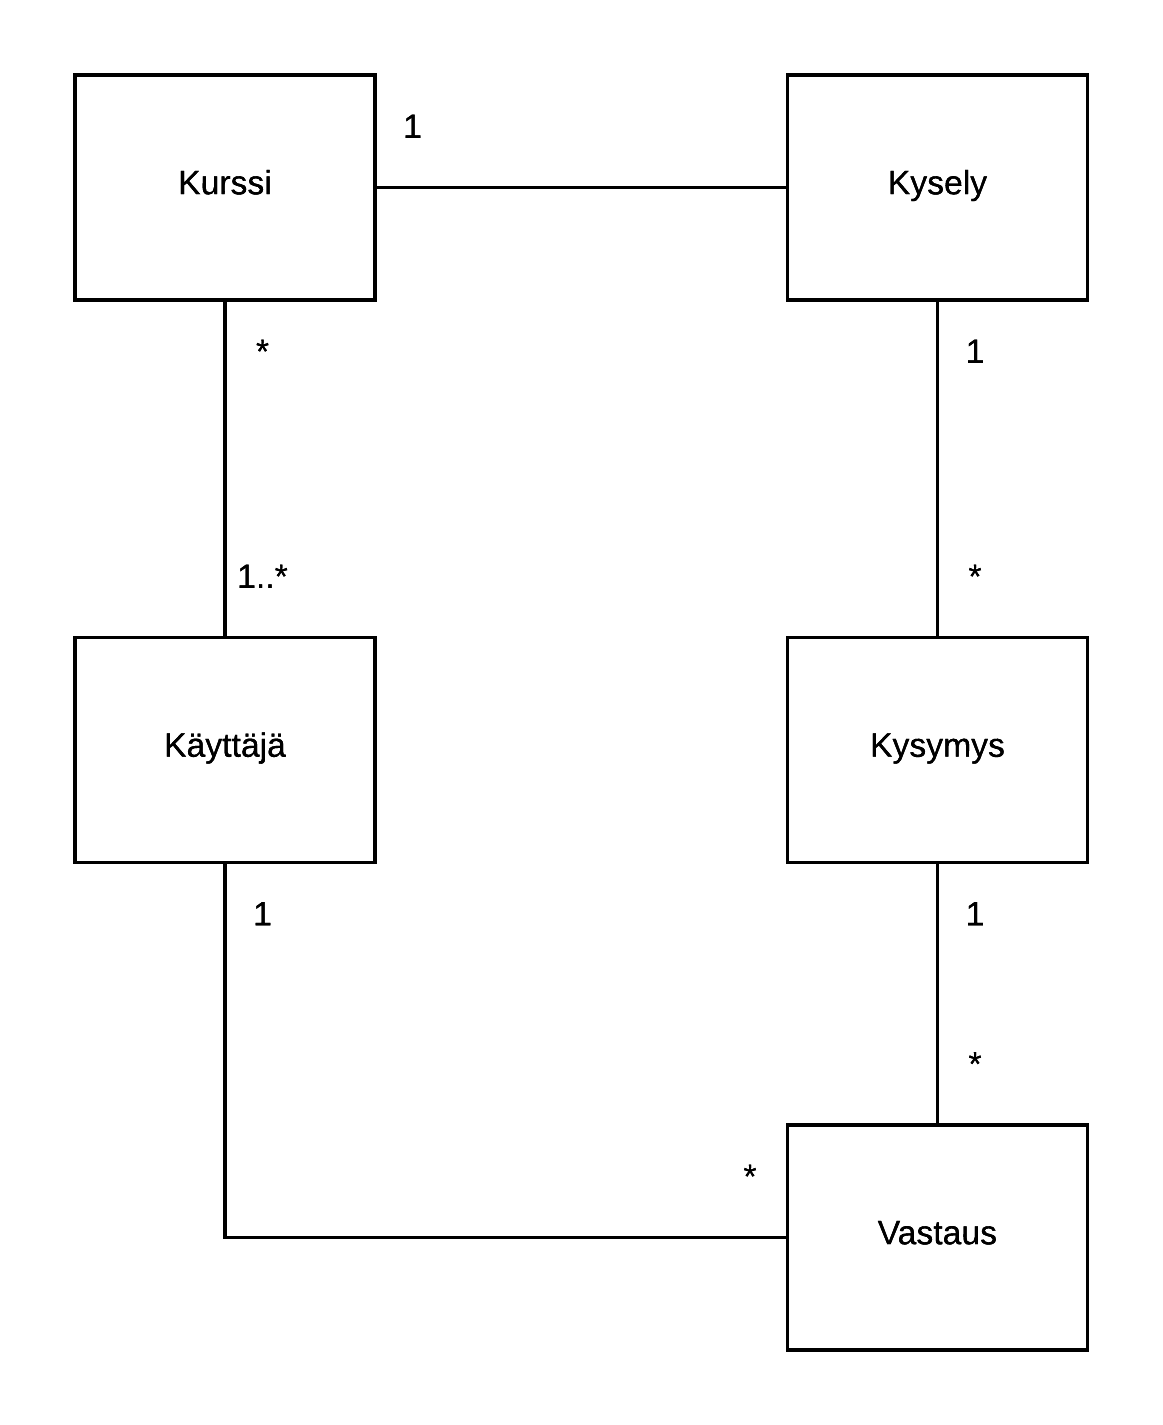
\includegraphics[width=\textwidth]{kuvat/kasitekaavio.png}
   \caption{Käsitekaavio järjestelmään tallennettavasta tiedosta}\label{fig:kasitekaavio}
\end{figure}

Järjestelmän tietosisältö on esitetty kuvassa \ref{fig:kasitekaavio}. Tarkemmat esittelyt kustakin käsitekaavion tietokohteesta ovat nähtävissä alla sekä taulukoissa \ref{tietokohde_ensimmainen}--\ref{tietokohde_viimeinen}.

Kukin järjestelmän käyttäjä kuuluu vähintään yhteen käyttäjäryhmään, joita ovat esimerkiksi opiskelija ja opettaja. Käyttäjäryhmän lisäksi jokainen henkilö kuuluu johonkin organisaatioon. Näitä ovat esimerkiksi eri laitokset sekä tiedekunta. Hallintohenkilöiden ja opettajien osalta organisaatio määräytyy työsopimuksen perusteella ja opiskelijoilla pääaineen. Tietokanta on suunniteltu sellaiseksi, että saman käyttäjän kuuluminen useaan käyttäjäryhmään ja/tai organisaatioon (esimerkiksi opettaja tietojenkäsittelytieteen laitoksella ja opiskelija fysiikan laitoksella) on mahdollista, mutta tämän työn puitteissa ei todennäköisesti ole ajankäytöllisesti järkevää toteuttaa tukea myös ohjelmalogiikalle.

Kysely edustaa tietyn kurssin palautekyselyä. Kyselyn tilat on tallennettu erilliseen tauluun, jotta tilojen nimitykset on helppo pitää konsistentteina muutoksista huolimatta ja tilojen arvojoukko on helppo tarkastaa. Kutakin kurssia kohden on yksi korkeintaan yksi kysely ja kukin kysely voi koostua mielivaltaisestsa määrästä kysymyksiä. Kukin kysymys kuuluu joko yhteen kyselyyn (kurssikohtaiset kysymykset) tai yhteen organisaatioon (laitos- tai tiedekuntakohtaiset kysymykset).

Kysely koostuu kysymyksistä, joita voi olla mielivaltainen määrä. Kukin kysymys kuuluu kuitenkin vain yhteen kurssiin tai organisaatioon. Kysymykset voivat olla vastaustyypiltään joko avoimia vai monivalintoja. Mikäli kyseessä on avoimen vastauksen kysymys, tallennetaan siihen saadut vastaukset AvoinVastaus-tauluun, jossa on yksi rivi kunkin opiskelijan kutakin vastausta kohden. Mikäli kyseessä on monivalinta, sisältää taulu Monivalintavastaus opiskelijan valitseman vastausvaihtoehdon järjestysluvun, jonka perusteella voidaan Monivalintavaihtoehto-taulusta hakea kyseistä vastausta vastaava selkokielinen teksti.


\begin{table}[h]
\caption{Käyttäjä} \label{tietokohde_ensimmainen}
\begin{tabularx}{\textwidth}{ | l X X |}
  \hline
  Attribuutti & Arvojoukko & Kuvailu \\
  \hline
  sähköposti & Merkkijono, korkeintaan 256 merkkiä & Käyttäjän sähköpostiosoite. Tätä käytetään viestinnän lisäksi kirjautumiseen. \\
  salasanaHash & Merkkijono, käytetystä salausalgoritmista riippuva maksimipituus tarkentuu myöhemmin. Tällä hetkellä käytössä 256. & Käyttäjän salasana suolattuna ja hashattynä\\
  suola & Merkkijono, käytetystä salausalgoritmista riippuva maksimipituus tarkentuu myöhemmin. Tällä hetkellä käytössä 16. & Käyttäjän salasanaa hashattaessa käytetty suola \\
  \hline
\end{tabularx}
\end{table}

\begin{table}[h]
\caption{Käyttäjäryhmä}
\begin{tabularx}{\textwidth}{|  l X X  |}
  \hline
  Attribuutti & Arvojoukko & Kuvailu \\
  \hline
   Nimi & Merkkijono, korkeintaan 150 merkkiä & Käyttäjäryhmän nimi, esimerkiksi "opiskelija" tai "opettaja" \\
  \hline
\end{tabularx}
\end{table}

\begin{table}[h]
\caption{Organisaatio}
\begin{tabularx}{\textwidth}{ |  l X X  |}
  \hline
  Attribuutti & Arvojoukko & Kuvailu \\
  \hline
  Nimi & Merkkijono, korkeintaan 150 merkkiä & Organisaation nimi, esimerkiksi "Matemaattis-luonnontieteellinen tiedekunta" tai "Fysiikan laitos" \\
  \hline
\end{tabularx}
\end{table}

\begin{table}[h]
\caption{Kurssi}
\begin{tabularx}{\textwidth}{ |  l X X  |}
  \hline
  Attribuutti & Arvojoukko & Kuvailu \\
  \hline
  Nimi & Merkkijono, korkeintaan 150 merkkiä & Kurssin nimi, esimerkiksi "Aineopintojen harjoitustyö: Tietokantasovellus (periodi II)" \\
  Kotisivu & Merkkijono, korkeintaan 500 merkkiä & Kurssin kotisivun URL. NULL, jos kurssilla ei ole kotisivua. \\
  Alkamispäivä & Date, ei päättymispäivää myöhemmin & Kurssin alkamispäivä \\
  Päättymispäivä & Date, ei alkamispäivää aiemmin & Kurssin päättymispäivä \\
  \hline
\end{tabularx}
\end{table}


\begin{table}[h]
\caption{Kysely}
\begin{tabularx}{\textwidth}{ |  l X X  |}
  \hline
  Attribuutti & Arvojoukko & Kuvailu \\
  \hline
  Kurssi & Viite kurssiin & Kurssi, johon kysely kuuluu. \\
  Tila & Viite tila-tauluun & Kurssin tämänhetkinen tila. \\
  \hline
\end{tabularx}
\end{table}

\begin{table}[h]
\caption{Kysymys}
\begin{tabularx}{\textwidth}{ |  l X X  |}
  \hline
  Attribuutti & Arvojoukko & Kuvailu \\
  \hline
  OrganisaatioID & Viite organisaatioon tai NULL & Viite organisaatioon, mikäli kyseessä on organisaatiokohtainen (laitos tai tiedekunta) kysymys \\
  KyselyID & Viite kyselyyn tai NULL & Viite kyselyyn, mikäli kyseessä on tiettyyn kyselyyn liittyvä kysymys \\
  Tyyppi & Merkkijono, korkeintaan 30 merkkiä & Kysymyksen tyyppi, joko "avoin" tai "monivalinta"\\
  Teksti & Merkkijono, korkeintaan 500 merkkiä & Opiskelijalle näytettävä kysymys \\
  \hline
\end{tabularx}
\end{table}

\begin{table}[h]
\caption{Avoin vastaus}
\begin{tabularx}{\textwidth}{ |  l X X  |}
  \hline
  Attribuutti & Arvojoukko & Kuvailu \\
  \hline
  OpiskelijaID & Viite opiskelijaan & Vastauksen antanut opiskelija \\
  KysymysID & Viite kysymykseen & Kysymys, johon vastaus liittyy \\
  Vastaus & Merkkijono, korkeintaan 2000 merkkiä & Opiskelijan antama vastaus \\
  \hline
\end{tabularx}
\end{table}

\begin{table}[h]
\caption{Monivalintavastaus}
\begin{tabularx}{\textwidth}{ |  l X X  |}
  \hline
  Attribuutti & Arvojoukko & Kuvailu \\
  \hline
  OpiskelijaID & Viite opiskelijaan & Vastauksen antanut opiskelija \\
  KysymysID & Viite kysymykseen & Kysymys, johon vastaus liittyy \\
  Järjestysluku & kokonaisluku & Monennenko vastausvaihtoehdon opiskelija on valinnut. Toimii foreign keynä yhdessä kysymysID:n kanssa \\
  \hline
\end{tabularx}
\end{table}

\begin{table}[h]
\caption{Monivalintavaihtoehto}
\begin{tabularx}{\textwidth}{ |  l X X  |}
  \hline
  Attribuutti & Arvojoukko & Kuvailu \\
  \hline
  KysymysID & Viite kysymykseen & Minkä kysymyksen vastausvaihtoehto on kyseessä \\
  Järjestysluku & kokonaisluku & Monesko kysymyksen vastauksista on kyseessä. Vaikuttaa järjestykseen, jossa vaihtoehdot esitetään opiskelijalle ja toimii osana primary keytä. \\
  Teksti & Merkkijono, korkeintaan 150 merkkiä & Teksti, joka opiskelijalle näytetään vastausvaihtoehtona \\
  \hline
\end{tabularx}
\end{table}

\begin{table}[h]
\caption{Tila} \label{tietokohde_viimeinen}
\begin{tabularx}{\textwidth}{ |  l X X  |}
  \hline
  Attribuutti & Arvojoukko & Kuvailu \\
  \hline
  Nimi & Merkkijono, korkeintaan 150 merkkiä & Teksti, joka kuvaa kyselyn tilaa\\
  \hline
\end{tabularx}
\end{table}

\section{Relaatiotietokantakaavio}
Käsitekaavion perusteella rakennettu relaatiokaavio on nähtävissä kuvassa \ref{fig:krelaatiokaavio}. Siihen on lisätty tarvittavat liitostaulut ja siinä ovat nähtävissä myös taulujen primary keyt (osalla erikseen lisätty ID, jota ei ole tarpeettomana sisällytetty käsitekaavion yhteydessä esitettyihin taulukoihin). Lisäksi kuvassa on esitetty taulujen primary ja foreign keyt.

\begin{figure}
   \centering
   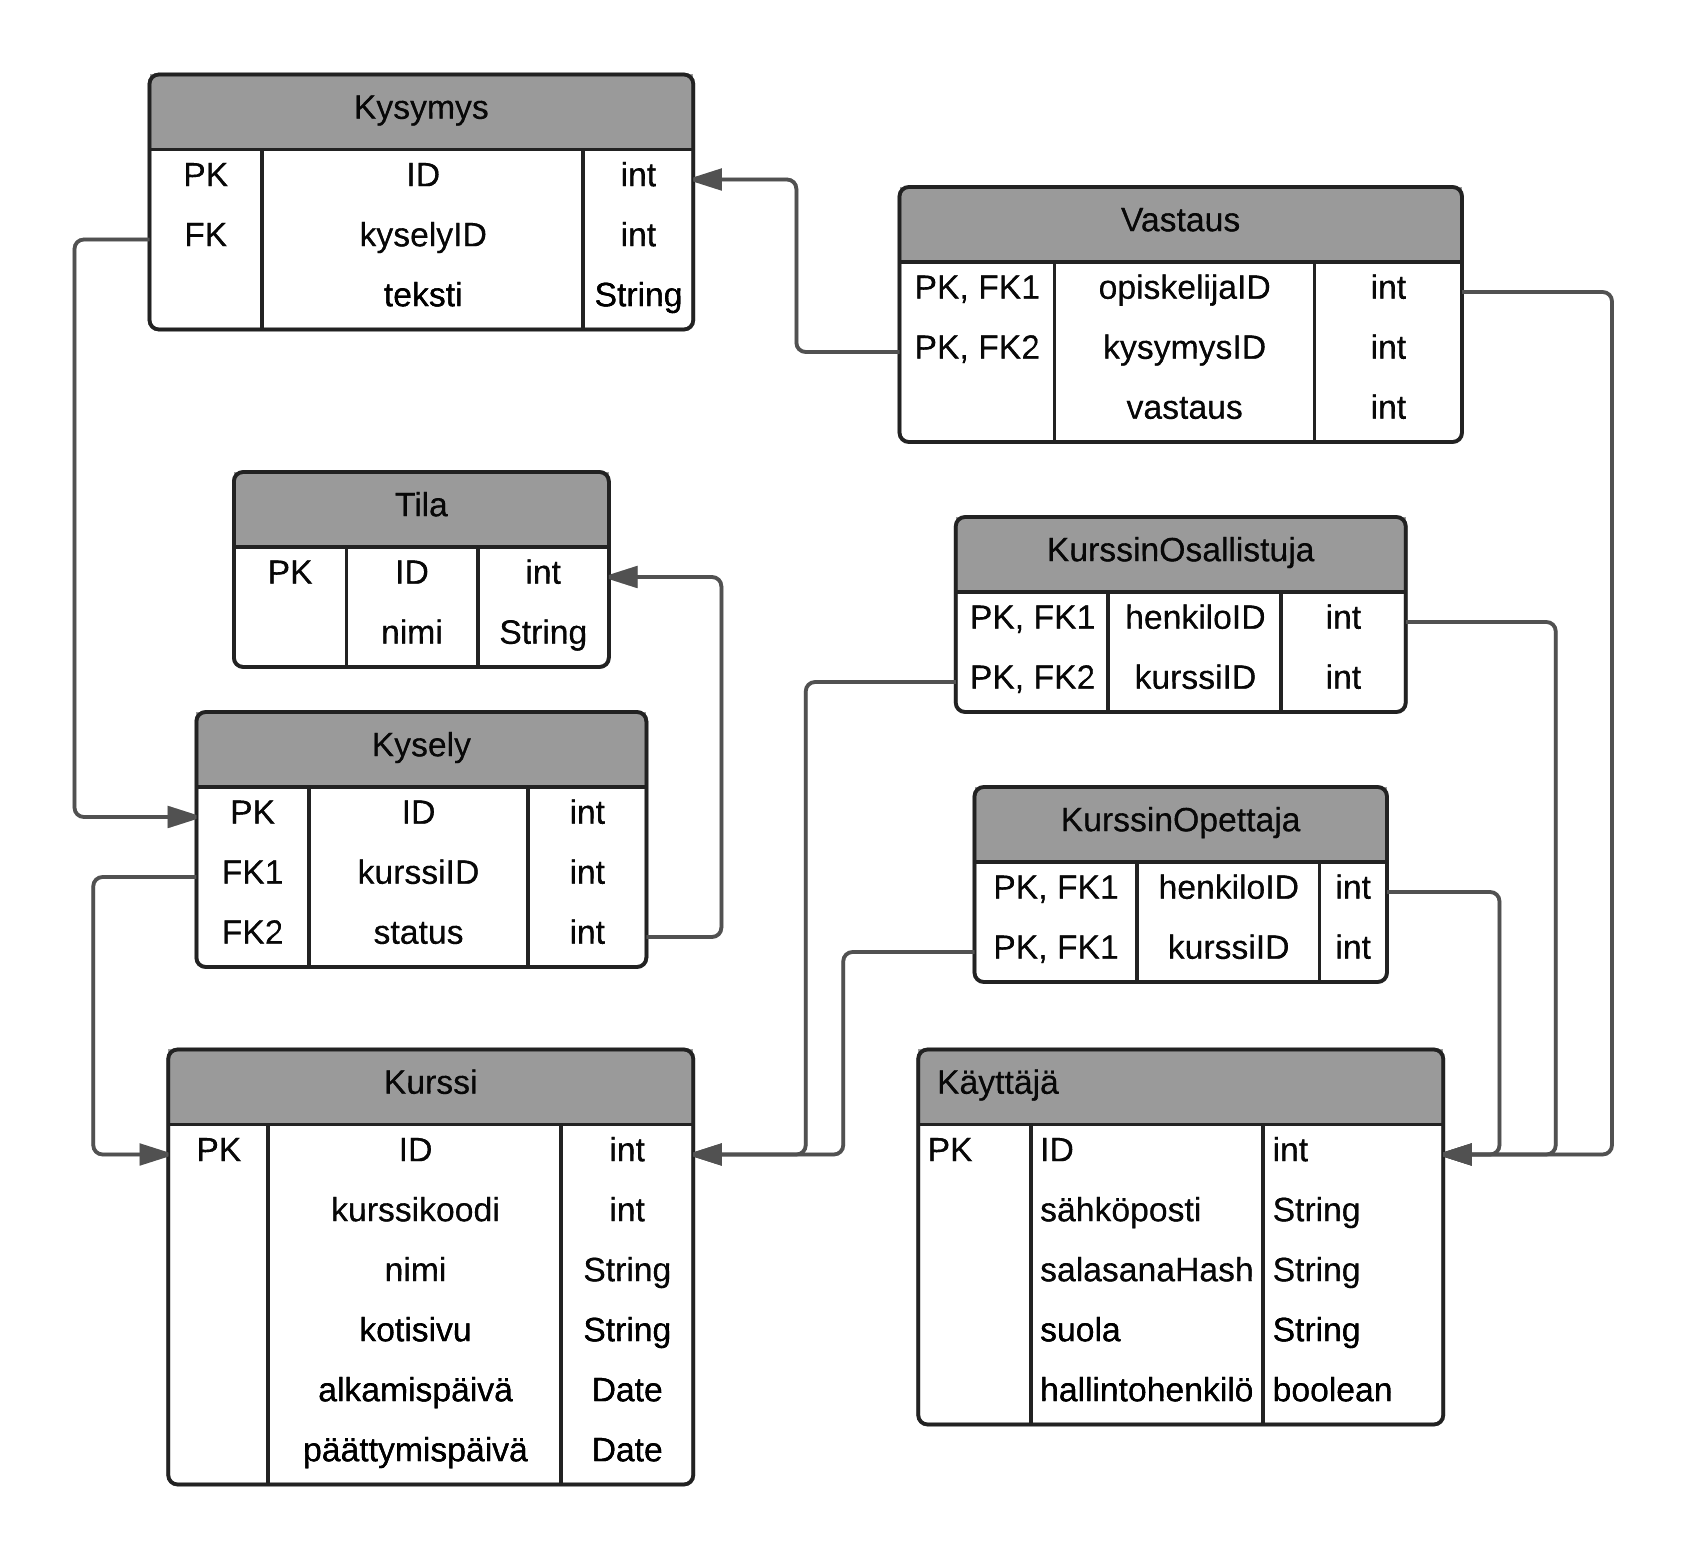
\includegraphics[width=\textwidth]{kuvat/relaatiokaavio-pysty.png}
   \caption{}\label{fig:krelaatiokaavio}
\end{figure}

\section{Järjestelmän yleisrakenne}

\section{Käyttöliittymä ja järjestelmän komponentit}

\section{Asennustiedot}

\section{Käynnistys- ja käyttöohje}



%%%%% Sisältö loppuu, lähdeluettelo %%%%%
\bibliographystyle{plain}
\small
\bibliography{lahteet}

\appendix
%\newpage
\section{Tärkeä liite}
Lorem ipsum.
\newpage



\end{document}
